
\section{Interlude: Piecewise-linear functions} 

\subsection*{Late parking ticket}

Mallory is having a miserable time.  A few weeks back she forgot to pay the parking meter and the city issued a parking ticket.  The parking ticket was for \$45 and was due within 30 days.  After that, the city imposes a late fee of \$10.  Bummer.

But Mallory is curious -- how can she write an equation to describe the cost of her parking ticket when it changes like that? She knows variables are 
$$D = \text{ time since she got the ticket (days) } \sim \text{ indep}$$
$$C = \text{ cost of parking ticket (\$) } \sim \text{ dep}$$
The starting amount (intercept) is \$45.  What's the rate of change (slope)?  During the first 30 days, the price does not change.  Since that rate of change is constant, we have a linear equation and the slope is \$0/day.  The equation for the first 30 days is
$$C = 45 + 0D$$
But $0D = 0$, so really
$$C = 45$$

By the way, there is a name for this type of function. It's called a \textbf{constant function}.  Meaning the value of the ticket is constant, at least during those first 30 days.

Now, after 30 days, the price jumps to $45+10 = \$55$.  The equation for the price then is
$$P = 55$$
another constant function.

There's a notation we can use to describe $C$ as a function of $D$ that includes both values.  We write
    $$C = \left\{ 
        \begin{array} {cl} 
            45 & \text{if } 0 \le D \le 30 \\
            55 & \text{if } D > 30
        \end{array}
    \right.$$

The way we read this notation is: if the number of days $D$ is between 0 and 30, then the ticket costs $P=$\$45 but if the number of days is over 30, then the ticket costs $C=$\$55.

\subsection*{Piecewise-linear functions and their graphs}

When our equation has two (or more) pieces, it's called a \textbf{piecewise-defined function}.  In this type of situation where both pieces are linear, it's called a \textbf{piecewise-linear function}.

What does the graph of a piecewise-linear function look like?  Let's make a table of values. Notice any value of $D$ over 30 days is gonna cost Mallory \$55.  Even if she's 2 minutes late, it's gonna cost \$55.  Note that 2 minutes late is 30.0014 days since 
$$ 2 \text{ min}  = \frac{2 \text{ min}}{1} \times  \frac{1 \text{ hour}}{60 \text{ min}}\times \frac{1 \text{ day}}{24 \text{ hours}} = 2 \div 60 \div 24 = .001388\ldots \approx .0014 \text{ days}$$

Here are the values we know.
\begin{center}
\begin{tabular}{c|c|c|c|c|c|c|c}
    $D$ & 0 & 10 & 20 & 30 & 30.0014 & 40 & 50 \\ \hline
    $C$ & 45 & 45 & 45 & 45 & 55 & 55 & 55
\end{tabular}
\end{center}

When we draw the graph and connect the dots into lines, we notice two things. First, the lines are horizontal.  That always happens when the function is constant and the slope is 0.  Second, there's a jump at 30 days where the graph isn't connected, which makes sense because the cost of the ticket jumps up after 30 days.

\begin{center}
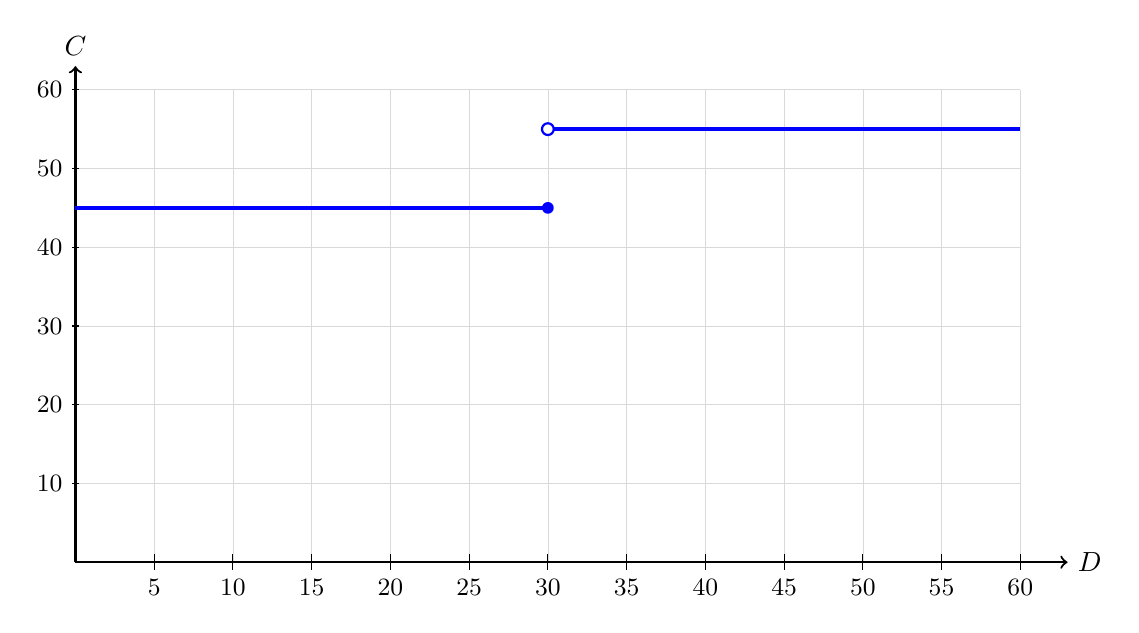
\begin{tikzpicture}[xscale=0.2, yscale=0.1]
    % Draw horizontal grid lines every 10 units along W (up to 90)
    \foreach \y in {10,20,...,60} {
        \draw[gray!30, very thin] (0,\y) -- (60,\y);
    }
    % Draw vertical grid lines every 1 unit along S (up to 20)
    \foreach \x in {5,10,...,60} {
        \draw[gray!30, very thin] (\x,0) -- (\x,60);
    }
    % Draw axes with tick marks and labels
    \draw[thick, ->] (0,0) -- (63,0) node[right] {$D$};
    \draw[thick, ->] (0,0) -- (0,63) node[above] {$C$};
    % X-axis tick marks every 1 up to 20
    \foreach \x in {5,10,...,60} {
        \draw (\x, 1) -- (\x, -1) node[below] {\small \x};
    }
    % Y-axis tick marks every 10 up to 90
    \foreach \y in {10,20,...,60} {
        \draw (0.2, \y) -- (-0.2, \y) node[left] {\small \y};
    }
    % Plot the line W = 45 from S = 0 to 30
    \draw[very thick, blue] plot[domain=0:30] (\x, {45});
    \draw[very thick, blue] plot[domain=30.2:60] (\x, {55});


    % Closed circle at (30, 45)
    \node[circle, fill=blue, inner sep=1.5pt] at (30, 45) {};

    % Open circle at (30, 55)
    \node[circle, draw=blue, fill=white, thick, inner sep=1.5pt] at (30, 55) {};
\end{tikzpicture}
\end{center}

Notice how we indicate the values corresponding to $D=30$.  We use a solid dot at $(30,45)$ because that's a point on the graph: at 30 days the parking ticket costs \$45.  We use an open dot at $(30,55)$ because that's not a point on the graph: at 30 days the parking ticket is not yet \$55. 

\subsection*{Late rent}

Mallory's troubles aren't over.  She's also behind on the rent.  She normally owes $900$ and there's a one week grace period, meaning she can pay up to one week late without any late fees.  For the next week, the late fee is \$10/day.  After that, the late fee jumps to \$25/day. 

Let's measure time in days. We have
$$L = \text{ how late the rent is (days)} \sim \text{ indep}$$
$$R = \text{ rent plus any late fees (\$)} \sim \text{ dep}$$

What happens during the first week?  For example, when $L=0$ days, the rent is \$900.  When $L=4$ days, we're within the grace period ($0 \le L \le 7$) so the rent is still \$900.  The equation during this week is $R = 900$.

What happens during the second week?  For example, when $L = 10$ days, she's $10-7=3$ days late and we're during the week where it costs an extra \$10/day ($7<L\le14$), so the rent is now 
\begin{eqnarray*}
  R & = & 900 + (10-7)\times 10 \\
  & = & 900 + 3\times 10 \\
  & = & 900 + 30 \\
  & = & \$930  
\end{eqnarray*}
The number of days late after the 7 day grace period is $L-7$.  The equation is 
$$R = 900 + (L-7)10$$
We can use the distributive property to multiply out to get
\begin{eqnarray*}
    R & = & 900 + (L-7)10 \\
    & = & 900+10L - 70 \\
    & = & 830+10L
\end{eqnarray*}

What happens during the third week?  For example, when $L=20$ days, she pays \$900 rent plus \$10/day for the first 7 days late plus \$25/day for the next $20-14=6$ days late, so that's a total of 
\begin{eqnarray*}
  R & = & 900 + 7 \times 10 + (20-14) \times 25 \\
    & = & 900 + 70 + 6 \times 25 \\
    & = & 970 + 150 \\
    & = & \$1120
\end{eqnarray*}
Ouch!
The number of days where she's gonna pay an extra \$25/day is $L -14$.  The equation is
$$R = 900 + 10\times7 + 25(L-14) $$
Again, we can use the distributive property to multiply out to get
\begin{eqnarray*}
    R & = & 900 + 10\times7 + 25(L-14) \\
    & = & 900 + 70 + 25L -25\times 14 \\
    & = & 970 + 25L - 350 \\
    & = & 620 + 25L
\end{eqnarray*}

When we put everything together we get

$$R = \left\{
    \begin{array}{cl}
        900 & \text{if } 0 \le L \le 7\\
        830 + 10L & \text{if } 7 < L \le 14\\
        620+25L& \text{if } L > 14 
    \end{array}
\right.
        $$

In case you were wondering about part days, Mallory's apartment complex  prorates the late fees are prorated by the hour (or even by the minute). So, for example, if Mallory pays her rent 9 days and 6 hours late, we would pay \$10/day for those 2 days and 6 hours after the grace period which is
\begin{eqnarray*}
  2 \text{ days} + 6 \text{ hours}
& = & 2 \text{ days} + \frac{6 \text{ hours}}{1} \times \frac{1 \text{ day}}{24 \text{ hours}} \\
& = & 2+6 \div 24 \\
& = & 2 + .25 = 2.25 \text{ days}  
\end{eqnarray*}
and so the late fee would be prorated at $2.25 \times 10 = \$22.50$ for a total of $900 + 22.50 = \$922.50$.

Let's summarize our examples and a few more values in a table.
\begin{center}
    \begin{tabular}{c||c|c|c||c|c||c|c|c}
        $L$ & 0 & 4 & 7 & 10& 14& 15 & 20\\ \hline
        $R$ & 0 & 900 & 900 & 930 & 970 & 995 & 1120 \\
    \end{tabular}
\end{center}

Now we can draw the graph.

\begin{center}
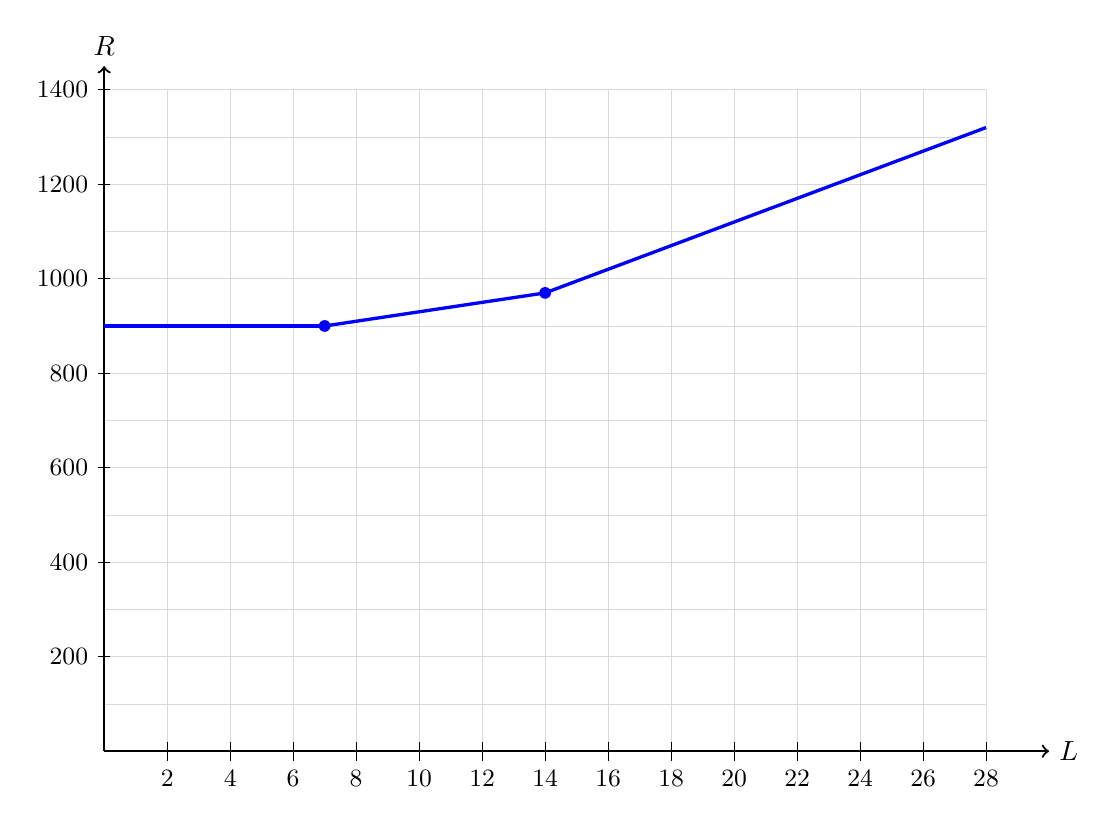
\begin{tikzpicture}[xscale=0.4, yscale=0.6]
    % Draw horizontal grid lines
    \foreach \y in {1,2,...,14} {
        \draw[gray!30, very thin] (0,\y) -- (28,\y);
    }
    % Draw vertical grid lines (fixed: 2..28 instead of ...28)
    \foreach \x in {2,4,...,28} {
        \draw[gray!30, very thin] (\x,0) -- (\x,14);
    }
    % Draw axes with tick marks and labels
    \draw[thick, ->] (0,0) -- (30,0) node[right] {$L$};
    \draw[thick, ->] (0,0) -- (0,14.5) node[above] {$R$};
    
    % X-axis tick marks (fixed: 2..28 instead of ...28)
    \foreach \x in {2,4,...,28} {
        \draw (\x, 0.2) -- (\x, -0.2) node[below] {\small \x};
    }
   % Y-axis tick marks labeled in hundreds (fixed: renamed \label to \lbl)
    \foreach \y/\lbl in {2/200, 4/400, 6/600, 8/800, 10/1000, 12/1200,14/1400} {
        \draw (0.2, \y) -- (-0.2, \y) node[left] {\small \lbl};
    }
    % Plot the line segments
    \draw[very thick, blue] plot[domain=0:7] (\x, {900/100});
    \draw[very thick, blue] plot[domain=7:14] (\x, {(830+10*\x)/100});
    \draw[very thick, blue] plot[domain=14:28] (\x, {(620+25*\x)/100});

    % Closed circles
    \node[circle, fill=blue, inner sep=1.5pt] at (7, 9) {};
    \node[circle, fill=blue, inner sep=1.5pt] at (14, 9.7) {};
\end{tikzpicture}
\end{center}

Notice that there are no jumps in the graph this time. That's because when $L=7$ we know $R=900$ but if we were to use the equation $R=830+10L$ when $L=7$ instead, we would get $R = 830+10 \times 7 = 900$ again.  That tells us that the second line starts where the first horizontal line ends. Similarly, when $L=14$ we use the equation $R = 830+10L$ to get $R = 830+10*14=970$ but if we were to use the equation $R=620+25L$ when $L = 14$ instead, then we would get $R=620+25 \times 14 = 970$ again. This tells us that the third line starts where the second line ends.  Sometimes we put closed dots to emphasize where the formula changes. 

 \input{GoDoWS}

\noindent \textbf{Do you know \ldots}

\begin{itemize}
\item Why we might model a situation using a piecewise-linear function?
\item How to model a situation using a piecewise-linear function?
\item What a constant function is and what its graph looks like?
\item How to graph a piecewise-linear function?
\item How to indicate jumps in the graph of a piecewise-linear function using open and closed points?
 \input{NotSure} 
\end{itemize}

\subsection*{Exercises}

\begin{enumerate} 
% WORKBOOK

\item A new bikeshare program rents e-bikes for the flat rate of \$10 for up to 30 minutes plus 20\textcent/minute thereafter. 
\begin{enumerate}
    \item What does it cost to rent an e-bike for 45 minutes?
    \item Name the variables, including units, and write a piecewise-linear equation illustrating the dependence. Hint: for times over 30 minutes you'll have to subtract 30 minutes before multiplying by 20\textcent/minute
    \item Draw a graph illustrating the dependence.  Include values from 0 to 2 hours.

\begin{center}
\scalebox {.8} {
\includegraphics [width = 6in] {Graphics/GraphPaper.jpg}}
\end{center}

\end{enumerate}

\item A food delivery app pays drivers a base rate of $\$1.20$ per mile for the first 5 miles of a delivery. To encourage long-distance deliveries, deliveries with a distance beyond 5 miles pay a bonus rate of $\$1.80$ per mile (for the miles over 5 miles).
\begin{enumerate}
    \item What does a 3 mile delivery pay? A 5 mile delivery?
    \item What does an 8 mile delivery pay?  20 mile delivery?  Note: your calculations should include $8-5$ and $20-5$.
    \item Name the variables, including units, and write a piecewise-linear equation illustrating the dependence.
    \item Draw a graph showing the pay for deliveries up to 20 miles.  Hint: When you use 5 miles in the equation for over 5 miles you should get the same pay as you found for 5 miles in (a) meaning that the graph does not jump.

\begin{center}
\scalebox {.8} {
\includegraphics [width = 6in] {Graphics/GraphPaper.jpg}}
\end{center}

\end{enumerate}

\item Seawater is naturally slightly basic (the opposite of acidic), at a pH of around 8.1.  To understand how carbon dioxide ($\text{CO}_2$) makes seawater more acidic (lower pH), Ngene has designed an experiment.  She slowly bubbles carbon dioxide ($\text{CO}_2$) gas into a small container of seawater.  At first, an active chemical buffer in the seawater slows down the drop in pH (which measures the acidity of the water). For the first $10\ \text{mL}$ of dissolved $\text{CO}_2$, the seawater's pH drops slowly at a rate of $0.02\text{ pH units per mL}$. (Note: mL stands for milliliter, which is 1/1000th of a liter.  The quanity 10mL is about 2 teaspoons.). Once the buffer capacity is exhausted beyond $10\ \text{mL}$, the pH drops rapidly at a steeper rate of $0.12\text{ pH units per mL}$ making the seawater more and more acidic.  Let's use the variables
    $$G = \text{ amount of carbon dioxide gas (mL) } \sim \text{indep}$$
    $$A = \text{ acidity of seawater (pH) } \sim \text{ dep}$$
\begin{enumerate}
    \item At the point where Ngene has bubbled 5 mL of $\text{CO}_2$ into the container of seawater, what is the pH?
    \item At the point where Ngene has bubbled 10 mL of $\text{CO}_2$ into the container of seawater, what is the pH?
    \item Write an equation for $A$ as a a function of $G$ for $0 \le G \le 10$. Hint: What is the starting pH?  What is the slope?  Another hint: The slope is negative.
    \item At the point where Ngene has bubbled 20 mL of $\text{CO}_2$ into the container or seawater, what is the pH?
    \item Write an equation for $A$ as a function of $G$ for $G > 10$.  Note that the starting value equals your answer from (b) and the slope of -0.12 pH units per mL applies to the amount of gas above 10mL, which is $G-10$.
    \item Use the distributive property to simplify your answer to (e).
    \item Write a piecewise-linear function illustrating how pH of Ngene's container of seawater depends on the amount of $\text{CO}_2$ she introduces.
\end{enumerate}

\item Oh, dear.  Mallory's having a very bad month.  She just realized a book she borrowed from the library is overdue.  The library has a grace period of 30 days followed by a fine of 10\textcent/day to a max of \$5. Notice that books are normally free to borrow from the library, so for up to 30 days late it costs \$0.
\begin{enumerate}    
    \item What will Mallory owe if the book is 20 days late?  40 days late?  2 months late? (Use 1 month = 30 days).
    \item Name the variables, including units.
    \item Write an equation illustrating the dependence, for late fees up to \$5.
    \item How many days late is a book that is first charged \$5?  Hint: try guessing.  If that doesn't work, solve your equation from (c).
    \item Write a piecewise-linear equation illustrating the dependence, for all possible days late.
\end{enumerate}

%% HOMEWORK

\item Tensia planted seeds outside once there was no chance of frost.  The seeds start sprouting once it's warm enough. The growth of a plant is measured in percentage of its size and plants grow faster on days where the temperature is is warmer.   For example, her plant might grow 5\% in a day at temperature that's on the cool side, but 20\% in a day where the temperature is warmer. She writes an equation describing the seed growth using the variables
$$T = \text{ temperature } (^\circ\text{F}) \sim \text{ indep}$$
$$G = \text{ daily growth rate } (\%) \sim \text{ dep}$$
Her equation is
$$G = \left\{
        \begin{array}{cl}
            0 & \text{if } 0 \le T \le 50 \\
            5(T-50) & \text{if } T>50
        \end{array}
    \right.$$
\begin{enumerate}
    \item At what temperature do Tensia's seeds sprout?  Hint: That would mean the growth is greater than 0.
    \item By what percentage do Tensia's seeds grow each day when the temperature is $60^\circ$F?  $75^\circ$F?
    \item Is there a jump in the graph?  Hint: what would the equation $G=5(T-50)$ give when $T=50$?
    \item Draw a graph illustrating the function.
\end{enumerate}

\item Pachak is boiling water to make some ramen noodles. He fills the pot with a couple of cups of cold tap water which is $15^\circ\text{C}$ (about $60^\circ\text{F}$). Next, he sets the pot on the stove and turns on the burner.  The burner adds thermal energy measured in kilojoules (kJ) to the water. For every kilojoule of heat the water absorbs, its temperature rises by about $0.8^\circ\text{C}$ until it hits $100^\circ\text{C}$ (or $212^\circ\text{F}$). After that, any extra energy goes into turning the boiling water into steam instead of making the water any hotter.
The variables in this story are 
$$E = \text{ energy from the burner (kJ)} \sim \text{ indep} $$
$$T = \text{ temperature of water } (^\circ \text{C}) \sim \text{ dep} $$
(It's not important for our story, but in case you're curious a typical high burner emits about 2 kJ/second, so it would emit 30 kJ after 15 seconds, 60 kJ after 30 seconds, and 120 kJ after 1 minute.)
\begin{enumerate}
    \item Write the linear equation that describes how the temperature of the water depends on the energy from the burner, for temperatures below boiling.
    \item According to your equation, what is the temperature of the water the burner has emitted 30kJ?  After 60 kJ?
    \item What does the equation say the temperature of the water is after the burner has emitted 120kJ of energy?  Why is this temperature incorrect?
    \item At what energy level does the water boil?  Hint: Solve your equation from (a) when $T=100$.
    \item Write the constant equation that describes the temperature of the water once it's reached the energy level you found in (d).
    \item Write a piecewise-linear equation that describes how the temperature of the water depends on the energy from the burner.
    \item Graph the function, including values up to at least 120kJ of energy.
\end{enumerate}



% Other possible examples for exercises

% calories per hour

\end{enumerate}

\bigskip

\noindent \textbf{When you're done \ldots}

\begin{itemize}
\item Don't forget to check your answers with those in the back of the textbook. 
\item Not sure if your answers are close enough? Compare with a classmate or ask the instructor.  
\item Getting the wrong answers or stuck on a problem?  Re-read the section and try the problem again.   If you're still stuck, work with a classmate or go to your instructor's office hours.
\item It's normal to find some parts of some problems difficult, but if all the problems are giving you grief, be sure to talk with your instructor or advisor about it.  They might be able to suggest strategies or support services that can help you succeed.
\item Make a list of key ideas or processes to remember from the section.  The ``Do you know?'' questions can be a good starting point.
\end{itemize}



